\documentclass[12pt,a4paper]{extarticle} %,twoside

\usepackage[nocolor]{derradeiro}

\definecolor{light-gray}{gray}{0.95}
\definecolor{mymauve}{rgb}{0.58,0,0.82}
\definecolor{mygreen}{rgb}{0,0.4,0}
\definecolor{mygray}{rgb}{0.5,0.5,0.5}
\lstset{basicstyle=\small, backgroundcolor=\color{light-gray}, showstringspaces=false, showspaces=false}
\begin{document}

\begin{titlepage}
\thispagestyle{empty}
\begin{center}\textsc{
Федеральное государственное бюджетное образовательное учреждение\\
высшего профессионального образования\\
<<САМАРСКИЙ ГОСУДАРСТВЕННЫЙ АЭРОКОСМИЧЕСКИЙ\\
УНИВЕРСИТЕТ имени академика С.П. КОРОЛЕВА
(национальный исследовательский университет)>>\\[50pt]
\textbf{Факультет информатики} \\[20pt]
\textbf{Кафедра технической кибернетики}}\\[30pt]
\textsc{
Пояснительная записка к лабораторной работе\\[30pt]
\large{Тема:<<\textbf{Метод Оцу}>>}\\[110pt]
}
\end{center}
\vfill
%~\hfill 
{\large
\begin{tabular*}{\textwidth}{@{\extracolsep{\fill}}ll}
	Выполнили студенты& Проценко В. И.\\
						    & Булдыгин Е.Ю.\\[10pt]
	Группа & 6128 \\[10pt]\\
\end{tabular*}
}
\vfill
\begin{center}
\large \today
\end{center}
\clearpage
\end{titlepage}
\newpage
\tableofcontents
\newpage

\section{Пороговая бинаризация методом Отсу}

    Бинарные изображения можно получать из полутоновых изображений посредством пороговой бинаризации. При выполнении этой операции часть пикселов выбирается в качестве пикселов переднего плана, представляющих объекты интереса, а остальные – в качестве фоновых пикселов. Зная распределение значений яркости на данном изображении, некоторые значения можно выбрать в качестве порогов, разделяющих пикселы на группы. В простейшем случае выбирается одно пороговое значение t. Все пикселы с яркостью больше или равной t становятся белыми, а остальные --- чёрными.\

    Для автоматического выбора порога бинаризации было разработано много различных методов. В данной работе реализован метод Отсу. Выбор порога в этом методе основан на минимизации внутригрупповой дисперсии двух групп пикселов, разделяемых оператором пороговой бинаризации. Отсу показал, что минимум внутригрупповой дисперсии обеспечивает максимум межгрупповой дисперсии (квадрат разности между средними значениями групп).
Интерпретируя гистограмму как частоту появления конкретного значения яркости, можно записать две величины:

\begin{equation*}
    p_1(t) = \frac{1}{| H |} \sum\limits_{i=0}^{t} H_i, \quad p_2(t)=1 - p_1(t) =  \frac{1}{| H |} \sum\limits_{i=t+1}^{255} H_i, \quad |H| = \sum\limits_{i=0}^{255} H_i,
\end{equation*}
где $p_i(t)$ --- вероятность класса, получаемая при бинаризации с порогом $t$. Значение порога в методе Отсу определяется как:
\begin{equation*}
    t= arg\max p_1(t)(1 - p_1(t))(\mu_1(t) - \mu_2(t))^2,
\end{equation*}
\begin{equation*}
     \mu_1(t) = \frac{1}{\sum\limits_{i=0}^t H_i} \sum\limits_{i=0}^t i H_i, \quad \mu_2(t) = \frac{1}{\sum\limits_{i=t+1}^{255} H_i} \sum\limits_{i=t+1}^{255} i H_i.
\end{equation*}

    Соответственно алгоритм заключается в простом переборе возможных пороговых значений t с выбором наилучшего, при этом все необходимые величины могут вычисляться рекуррентно.

    Таким образом, для реализации пороговой обработки методом Отсу необходимо провести вычисления в три этапа:
\begin{enumerate}
    \item сбор гистограммы яркости;\\
    \item расчёт порогового значения t;\\
    \item пороговая бинаризация с полученным порогом.
\end{enumerate}

\newpage
\section{Настройка оборудования} \label{sec:TuningCluster}
\subsection{Настройка одного узла}

    Для настройки одиночного узла не требуется прилагать огромных усилий. Подробное описание действий по устройству кластера на базе Hadoop можно найти по ссылкам:
\begin{enumerate}
    \item[] \href{http://www.michael-noll.com/tutorials/running-hadoop-on-ubuntu-linux-single-node-cluster/}{http://www.michael-noll.com/tutorials/running-hadoop-on-ubuntu-linux-single-node-cluster/}
    \item[] \href{http://www.michael-noll.com/tutorials/running-hadoop-on-ubuntu-linux-multi-node-cluster/}{http://www.michael-noll.com/tutorials/running-hadoop-on-ubuntu-linux-multi-node-cluster/}
\end{enumerate}

    Дальнейшее описание представляет собой краткий обзор этих статей. Для установки Hadoop необходимо:
\begin{enumerate}
    \item Компьютер с Ubuntu 12.04 LTS;
    \item Дистрибутив Hadoop 1.0.4;
    \item Свежая версия Java SDK (в данной работе был использован Java SE 1.7.0\_17);
    \item Настроенная SSH.
\end{enumerate}

    В случае установки Hadoop на чистую систему, необходимо установить Java SDK с сайта Oracle, так как предустановленный OpenJDK может не поддерживать некоторые элементы Hadoop.
\noindent Для начала удаляется OpenJDK и всё что с ним связано:
\begin{lstlisting}[language=sh]
    $ sudo apt-get purge openjdk*
\end{lstlisting}

\noindent Необходимый Java SDK можно скачать с сайта (для Ubuntu выбираем .tar.gz):
\begin{enumerate}
    \item[] \href{http://www.oracle.com/technetwork/java/javase/downloads/jdk7-downloads-1880260.html}{http://www.oracle.com/technetwork/java/javase/downloads/jdk7-downloads-1880260.html}
\end{enumerate}

\noindent Далее распаковываем скачанный архив и перемещаем содержимое в каталог /usr/lib/jvm/:
\begin{lstlisting}[language=sh]
    $ tar -xvf $HOME/Downloads/jdk-7u4-linux-x64.tar.gz
    $ mv $HOME/jdk1.7.0_04/ /usr/lib/jvm/
\end{lstlisting}

\noindent Hadoop использует протокол SSH для управления узлами, поэтому необходимо сначала установить SSH-сервер:
\begin{lstlisting}[language=sh]
    $ sudo apt-get install ssh
\end{lstlisting}

\noindent Для пользователя создаётся ключ для SSH-соединения (в данном случае пользователь hduser), который соответствует пустому паролю:
\begin{lstlisting}[language=sh]
    $ su - hduser
    $ ssh-keygen -t rsa -P ""
\end{lstlisting}

\noindent Затем открываем доступ к локальной машине с созданным ключом:
\begin{lstlisting}
    $ cat $HOME/.ssh/id_rsa.pub >> $HOME/.ssh/authorized_keys
\end{lstlisting}

\noindent Для проверки запускаем соединение с localhost, при этом он будет помещён в список известных хостов hduser:
\begin{lstlisting}[language=sh]
    $ ssh localhost
\end{lstlisting}

\noindent Следующим шагом является отключение IPv6. Для этого открываем файл /etc/sysctl.conf и добавляем в конец файла строки:
\begin{lstlisting}
    net.ipv6.conf.all.disable_ipv6 = 1
    net.ipv6.conf.default.disable_ipv6 = 1
    net.ipv6.conf.lo.disable_ipv6 = 1
\end{lstlisting}

\noindent После сохранения, можно проверить результат командой:
\begin{lstlisting}[language=sh]
    $ cat /proc/sys/net/ipv6/conf/all/disable_ipv6
\end{lstlisting}

    \noindentЕсли всё было правильно сделано, то увидим 1.

\noindent Теперь можно приступить  к установке Hadoop. Для этого скачиваем дистрибутив с официального сайта (http://hadoop.apache.org/)  и извлекаем содержимое в симпатичный нам каталог (например, в /usr/local/hadoop), при этом не стоит забывать о правах доступа (владельцем должен быть hduser и группа hadoop). Процесс можно выполнить командами:
\begin{lstlisting}[language=sh]
    $ sudo tar xzf $HOME/Downloads/hadoop-1.0.4.tar.gz
    $ sudo mv $HOME/hadoop-1.0.4 /usr/local/hadoop
    $ sudo chown -R hduser:hadoop /usr/local/hadoop
\end{lstlisting}

\noindent После этого необходимо обновить \$HOME/.bashrc в соответствии со следующими строками:
\begin{lstlisting}[language=sh]
    # Установка переменной, связанной с Hadoop
    export HADOOP_HOME=/usr/local/hadoop

    # Установка местоположения Java SDK
    export JAVA_HOME=/usr/lib/jvm/java-6-sun

    # Некоторые удобные псевдонимы и функции
    # для работы Hadoop, связаной с командами
    unalias fs &> /dev/null
    alias fs="hadoop fs"
    unalias hls &> /dev/null
    alias hls="fs -ls"

    # If you have LZO compression enabled in your 
    # Hadoop cluster and compress job outputs with 
    # LZOP (not covered in this tutorial):
    # C    onveniently inspect an LZOP compressed 
    # file from the command
    # line; run via:
    #
    # $ lzohead /hdfs/path/to/lzop/compressed/file.lzo
    #
    # Requires installed 'lzop' command.
    #
    lzohead () {
        hadoop fs -cat $1 | lzop -dc | head -1000 | less
    }

    # Добавляем Hadoop bin/ в PATH
    export PATH=$PATH:$HADOOP_HOME/bin
\end{lstlisting}

\noindent Теперь можно заняться конфигурированием одиночного узла. Для начала открываем файл /usr/local/hadoop/conf/hadoop-env.sh и заменяем строчку вида
\begin{lstlisting}[language=sh]
    # export JAVA_HOME=/usr/lib/j2sdk1.5-sun
\end{lstlisting}
на строчку с соответствующим указанием директории с Java SDK:
\begin{lstlisting}[language=sh]
    export JAVA_HOME=/usr/lib/jvm/java1.7.0_17
\end{lstlisting}

\noindent Можно создать отдельный каталог для служебного использования распределённой файловой системой (в нашем случае это будет /app/hadoop/tmp, не забываем при этом про права доступа):
\begin{lstlisting}[language=sh]
    $ sudo mkdir -p /app/hadoop/tmp
    $ sudo chown hduser:hadoop /app/hadoop/tmp
\end{lstlisting}

\noindent Открываем conf/core-site.xml в директории с Hadoop и между тегами <configuration> ... </configuration> добавляем следующие строки:
\begin{lstlisting}[language=xml]
    <property>
      <name>hadoop.tmp.dir</name>
      <value>/app/hadoop/tmp</value>
      <description>
        A base for other temporary directories.
      </description>
    </property>
    
    <property>
      <name>fs.default.name</name>
      <value>hdfs://localhost:54310</value>
      <description>The name of the default file system. 
        A URI whose scheme and authority determine the 
        FileSystem implementation.  The uri's scheme
        determines the config property (fs.SCHEME.impl) 
        naming the FileSystem implementation class.  
        The uri's authority is used to  determine the host,
        port, etc. for a filesystem.
      </description>
    </property>
\end{lstlisting}

\noindent В файле conf/mapred-site.xml между тегами <configuration> ... </configuration> добавляем:
\begin{lstlisting}[language=xml]
    <property>
      <name>mapred.job.tracker</name>
      <value>localhost:54311</value>
      <description>The host and port that the MapReduce 
      job tracker runs at.  If "local", then jobs are 
      run in-process as a single map and reduce task.
      </description>
    </property>
\end{lstlisting}

\noindent В файле conf/hdfs-site.xml между тегами <configuration> ... </configuration> добавляем (пока что у нас только один узел --- фактор репликации равен единице):
\begin{lstlisting}[language=xml]
    <property>
      <name>dfs.replication</name>
      <value>1</value>
      <description>Default block replication.
        The actual number of replications can
        be specified when the file is created.  
        The default is used if replication is 
        not specified in create time.
      </description>
    </property>
\end{lstlisting}

\noindent Теперь всё готово. Перед запуском форматируем HDFS командой из терминала:
\begin{lstlisting}[language=sh]
    $ /usr/local/hadoop/bin/hadoop namenode -format
\end{lstlisting}
\newpage
\noindent Если всё сконфигурировано правильно, то в терминале появятся примерно такие сообщения:
\begin{figure}[h!]
 \centering
    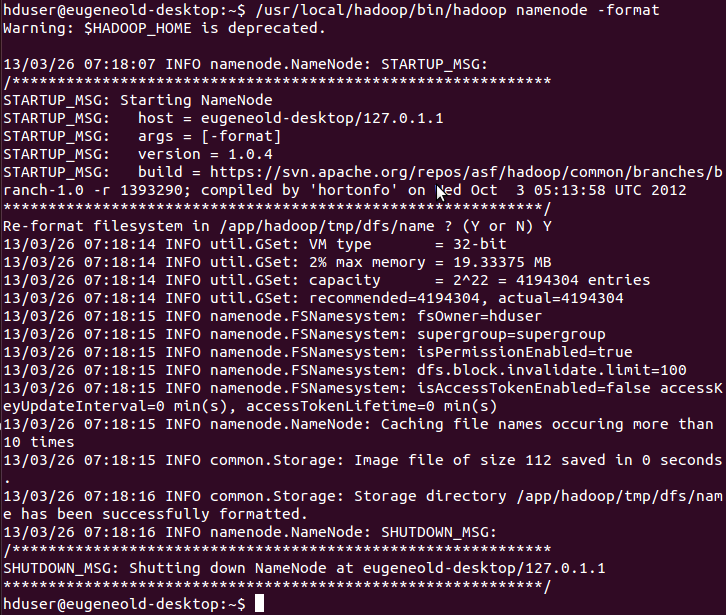
\includegraphics[width=0.7\textwidth]{images/1.png}
\end{figure}

\noindent Для запуска одноузлового кластера используется скрипт start-all.sh:
\begin{figure}[h!]
 \centering
    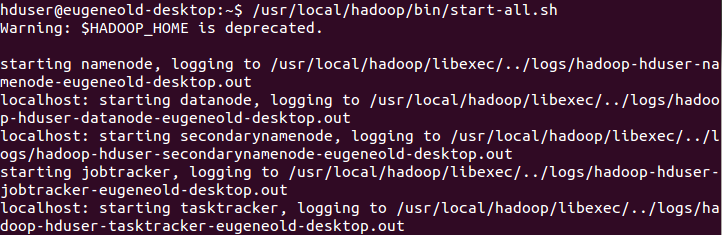
\includegraphics[width=0.7\textwidth]{images/2.png}
\end{figure}

\noindent Остановка кластера осуществляется скриптом stop-all.sh:
\begin{figure}[h]
 \centering
    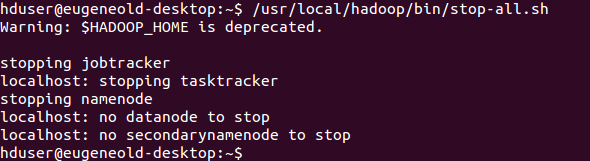
\includegraphics[width=0.7\textwidth]{images/3.png}
\end{figure}

\clearpage\newpage
\subsection{Настройка двухузлового кластера}

    Если в локальной сети есть два одноузловых кластера, настроенных по предыдущему пункту, то для объединения их в один двухузловой. Если компьютеры не являются членами локальной сети, но есть доступ в Интернет, то можно воспользоваться средствами построения VPN, например Hamachi.
    
    Для удобства работы вместо ip-адресов можно использовать символьные значения, для этого добавляем в файл /etc/hosts следующие строки (на обеих машинах):
\begin{lstlisting}
    192.168.0.1    master
    192.168.0.2    slave
\end{lstlisting}
	\textbf{Примечание.} Важно, чтобы имя компьютера совпадало с введёными сокращениями. В ходе установки было выяснено, что помимо перечисленных строчек, в hosts slave узла необходимо также добавить пару <<ip-адрес название удалённой машины>>, так как hadoop не мог разрешить имя компьютера и сопоставить ему адрес master узла.

 Для корректного функционирования Hadoop необходимо обеспечить SSH-соединение без ввода пароля. Для этого выполняем команду копирования ключа (создан в предыдущем разделе):
\begin{lstlisting}[language=sh]
    hduser@master:~$ ssh-copy-id -i $HOME/.ssh/id_rsa.pub hduser@slave
\end{lstlisting}

\noindent После этого проверяем соединения master-to-master и master-to-slave, при запросе подтверждаем продолжение соединения: 
\begin{lstlisting}[language=sh]
    hduser@master:~$ ssh master
    The authenticity of host 'master (192.168.0.1)' can't be established.
    RSA key fingerprint is 3b:21:b3:c0:21:5c:7c:54:2f:1e:2d:96:79:eb:7f:95.
    Are you sure you want to continue connecting (yes/no)? yes
    Warning: Permanently added 'master' (RSA) to the list of known hosts.
    Linux master 2.6.20-16-386 #2 Thu Jun 7 20:16:13 UTC 2007 i686
    
    hduser@master:~$ ssh slave
    The authenticity of host 'slave (192.168.0.2)' can't be established.
    RSA key fingerprint is 74:d7:61:86:db:86:8f:31:90:9c:68:b0:13:88:52:72.
    Are you sure you want to continue connecting (yes/no)? yes
    Warning: Permanently added 'slave' (RSA) to the list of known hosts.
\end{lstlisting}

\noindent На рисунке представлено различие между master и slave. Помимо этого, на master предполагается запуск скриптов start-dfs.sh и start-mapred.sh, которые запускают необходимых демонов во вторичных узлах.
\begin{figure}[h]
 \centering
    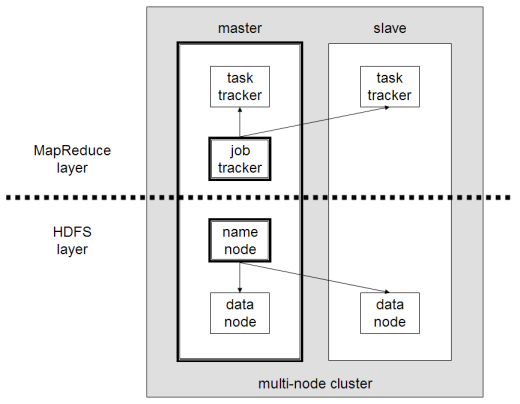
\includegraphics[width=0.5\textwidth]{images/two-node-cluster.png}
\end{figure}

\newpage
\noindent Для настройки узла-мастера необходимо добавить master в /conf/masters и пару строчек в /conf/slaves:
\begin{lstlisting}
    master
    slave
\end{lstlisting}

\noindent На всех узлах производим следующие модификации /conf/*-site. Как и прежде, между тегами <configuration> ... </configuration> нужно обновить содержимое в соответствии со следующим текстом:
\begin{enumerate}
    \item  Для conf/core-site.xml  на всех машинах:
\begin{lstlisting}[language=xml]
    <property>
      <name>fs.default.name</name>
      <value>hdfs://master:54310</value>
      <description>The name of the default file system.
      A URI whose scheme and authority determine 
      the FileSystem implementation. The uri's scheme 
      determines the config property (fs.SCHEME.impl) 
      naming the FileSystem implementation class. 
      The uri's authority is used to determine the host,
      port, etc. for a filesystem.
      </description>
    </property>
\end{lstlisting}
    \item Для conf/mapred-site.xml на всех машинах:
\begin{lstlisting}
    <property>
      <name>mapred.job.tracker</name>
      <value>master:54311</value>
      <description>The host and port that the MapReduce
      job tracker runs at.  If "local", then jobs are
      run in-process as a single map and reduce task.
      </description>
    </property>
\end{lstlisting}
    \item Для conf/hdfs-site.xml  на всех машинах:
\begin{lstlisting}[language=xml]
    <property>
      <name>dfs.replication</name>
      <value>2</value>
      <description>Default block replication.
      The actual number of replications can be specified 
      when the file is created. The default is used if 
      replication is not specified in create time.
      </description>
    </property>
\end{lstlisting}
\end{enumerate}

\noindent Теперь всё настроено, можно форматировать HDFS и запускать кластер. На master для форматирования файловой  системы вводим команду:
\begin{lstlisting}
    hduser@master$ /usr/local/hadoop/bin/hadoop namenode -format
\end{lstlisting}

\newpage
\noindent Запуск кластера проводится в два этапа:
\begin{enumerate}
    \item Запуск файловой системы:
    \begin{lstlisting}
    hduser@master$ /usr/local/hadoop/bin/start-dfs.sh
    \end{lstlisting}
    \item Запуск фоновых программ MapReduce (JobTracker на мастере и TaskTracker на обоих узлах):
    \begin{lstlisting}
    hduser@master$ /usr/local/hadoop/bin/start-mapred.sh
    \end{lstlisting}
\end{enumerate}

\noindent Успешность запуска можно проверить по соответствующим логам в logs/ в директории  с Hadoop или же запустить jps:
\begin{lstlisting}
    hduser@master$ $JAVA_HOME/bin/jps
    16017 Jps
    14799 NameNode
    15686 TaskTracker
    14880 DataNode
    15596 JobTracker
    14977 SecondaryNameNode
\end{lstlisting}

\noindent На компьютере slave:
\begin{lstlisting}
    hduser@slave$ $JAVA_HOME/bin/jps
    15183 DataNode
    15897 TaskTracker
    16284 Jps
\end{lstlisting}

\noindent Остановка кластера также происходит в два этапа:
\begin{enumerate}
    \item Остановка фоновых программ MapReduce:
    \begin{lstlisting}[language=sh]
    hduser@master$ /usr/local/hadoop/bin/stop-mapred.sh
    \end{lstlisting}
    \item Остановка файловой системы:
    \begin{lstlisting}[language=sh]
    hduser@master$ /usr/local/hadoop/bin/stop-dfs.sh
    \end{lstlisting}
\end{enumerate}

\newpage
\noindent Если сделать всё правильно, то получим примерный вывод (как легко заметить, вторичный узел в данном запуске называется old\_slave, если всё было сделано по инструкции, то вторичный узел должен иметь название slave):
\begin{figure}[h]
 \centering
    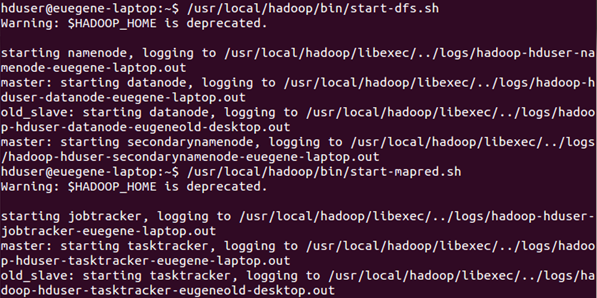
\includegraphics[width=0.9\textwidth]{images/4.png}
\end{figure}
\begin{figure}[h]
 \centering
    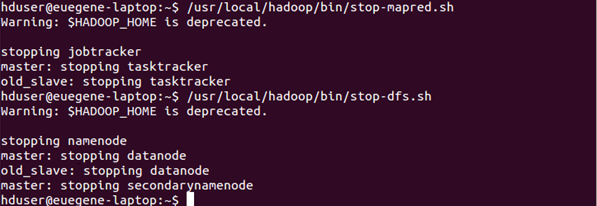
\includegraphics[width=0.9\textwidth]{images/5.png}
\end{figure}

\clearpage\newpage
\section{Описание проекта}
Структура проекта
\begin{lstlisting}    
    /src
    /lib
    /input
    build.xml
    buildrun.sh
    run.sh
\end{lstlisting}

    Проект поддерживает компиляцию под следующие архитектуры: linux i386, linux amd64, windows x86, windows x64. Скомпилированные версии тестировались в Windows 7 x64 c библиотекой Karmasphere: Hadoop MapReduce 0.20.203 и в Ubuntu (см. Версии использованного программного обеспечения, раздел \ref{sec:envsoft}) с версией Hadoop 1.0.4.

    Для компиляции необходимо установить ant и находясь в папке с проектом запустить его. Например, проект находится в linux в директории /develop/java/project, запускаем консоль, в ней вводим две команды: "cd  /develop/java/project", "ant".

\subsection{Описание программы}
    Листинги программы приведены в конце отчёта. За основу был взят код открытого проекта \href{http://code.google.com/p/hadoop-computer-vision/}{http://code.google.com/p/hadoop-computer-vision/}, а именно код примера Histogram.java.

    Программа состоит из двух фаз. Нахождение порогового значения и применения порога к изображению. На вход алгоритма подаются все изображения находящиеся в заданной папке. 

	\begin{figure}[h]
		 \centering
		 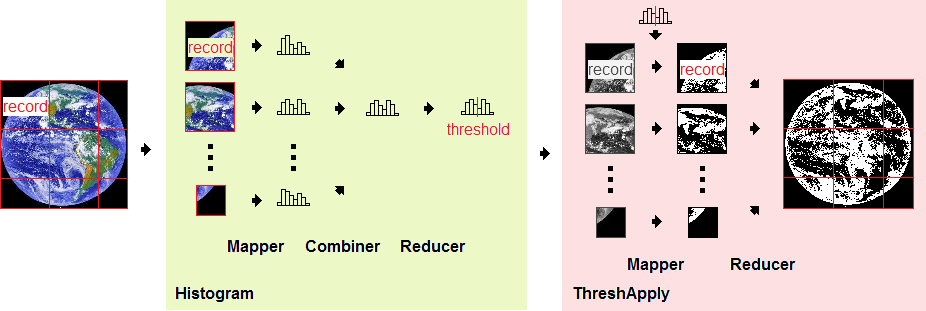
\includegraphics[width=\textwidth]{images/mapreducejob.png}
		 \caption{Схема работы алгоритма. Обработка одного изображения.}
	\end{figure}

    \textbf{Первая фаза} пробегает по изображениям. Метод getSplits() задаёт отображение: одному изображению соответствует один split, файлы являются не делимыми для InputReader. ImageRecordReader делит полученное изображение прямоугольными окнам на более мелкие изображения, теперь представляющие из себя единичные записи.\\[5pt]

	\begin{figure}[h]
		 \centering
		 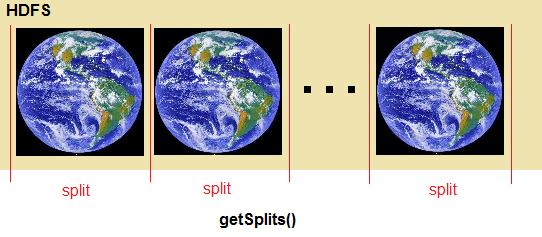
\includegraphics[width=0.6\textwidth]{images/getsplits.png}
		 \caption{Декомпозиция входного потока изображений. Метод getSplits().}
	\end{figure}

    \noindent \textbf{Map} класс подсчитывает частичные гистограммы для каждой записи. 

    \noindent Входные параметры map():
    \begin{itemize}
        \item[] \textit{Ключ} --- имя файла,
        \item[] \textit{Значение} --- объект типа Image, часть исходного изображения, соответствующая ключу.
    \end{itemize}

    \noindent Выходные параметры map():
    \begin{itemize}
        \item[] \textit{Ключ} --- имя файла,
        \item[] \textit{Значение} --- объект типа LongArrayWritable, частичная гистограмма.
    \end{itemize}

    \noindent \textbf{Combiner} класс подсчитывает итоговую гистограмму для всех значений ключа. 

    \noindent Входные параметры reduce():
    \begin{itemize}
        \item[] \textit{Ключ} --- имя файла,
        \item[] \textit{Значение} --- список значений типа LongArrayWritable, частичные гистограммы.
    \end{itemize}

    \noindent Выходные параметры reduce():
    \begin{itemize}
        \item[] \textit{Ключ} --- имя файла,
        \item[] \textit{Значение} --- объект типа LongArrayWritable, итоговая гистограмма.
    \end{itemize}

    \noindent \textbf{Reducer} класс подсчитывает итоговую гистограмму для всех значений ключа. 

    \noindent Входные параметры reduce():
    \begin{itemize}
        \item[] \textit{Ключ} --- имя файла,
        \item[] \textit{Значение} --- объект типа LongArrayWritable, итоговая гистограмма.
    \end{itemize}

    \noindent Выходные параметры reduce():
    \begin{itemize}
        \item[] \textit{Ключ} --- имя файла,
        \item[] \textit{Значение} --- текстовое значение подсчитанного порога.
    \end{itemize}

 \textbf{Вторая фаза} на вход получает те же изображения, что и первая фаза. Путь к каталогу с подсчитанными пороговыми значениями передаётся через конфигуранцию, класс Configuration, вызовом
 \begin{lstlisting}[language=Java]
    conf.setStrings("mapreduce.imagerecordreader.threshpath", args[1]) 
\end{lstlisting}
где args[1] --- временная папка. Декомозиция входного потока изображений такая же, как и в первой фазе.\\[5pt]

    \noindent \textbf{Map} класс находит пороговое значение для данного ключа--имени файла и применяет его к текущей записи.

    \noindent Входные параметры map():
    \begin{itemize}
        \item[] \textit{Ключ} --- имя файла,
        \item[] \textit{Значение} --- объект типа Image, часть исходного изображения, соответствующая ключу.
    \end{itemize}

    \noindent Выходные параметры map():
    \begin{itemize}
        \item[] \textit{Ключ} --- имя файла,
        \item[] \textit{Значение} --- объект типа Image, обработанная часть исходного изображения.
    \end{itemize}

    \noindent \textbf{Reducer} класс объединяет части  данного ключа в итоговое крупное изображение. 

    \noindent Входные параметры reduce():
    \begin{itemize}
        \item[] \textit{Ключ} --- имя файла,
        \item[] \textit{Значение} --- объект типа Image, обработанная часть исходного изображения.
    \end{itemize}

    \noindent Выходные параметры reduce():
    \begin{itemize}
        \item[] \textit{Ключ} --- имя файла,
        \item[] \textit{Значение} --- объект типа Image, обработанное исходное изображение.
    \end{itemize}

    

\subsection{Описание build.xml}
    Рассмотрим build скрипт.

\begin{lstlisting}[language=xml]
    <project  default="endpoint" 
              name="Create Runnable Jar for Project NewSandCastle" 
              basedir=".">
\end{lstlisting}
    
    Описываем создание проекта "Create Runnable Jar for Project NewSandCastle", текущий каталог - каталог расположения build.xml. Построение будет ждать завершения элемента с названием "endpoint" и всех зависимых элементов.
\begin{lstlisting}[language=xml]
    <property name="src" location="src"/>
    <property name="build" location="build"/>
    <property name="lib" location="lib"/>    
    <property name="jarname" location="MethodOzu.jar"/>
\end{lstlisting}

    Устанавливаем необходимые переменные.
\begin{lstlisting}[language=xml]
    <condition property="isWindows86">
        <and>
            <os family="windows"/>
            <or>
                <equals arg1="${os.arch}" arg2="i386"/>
                <equals arg1="${os.arch}" arg2="x86"/>
            </or>
        </and>
    </condition>
    <condition property="isWindows64">
        <and>
            <os family="windows"/>
            <or>
                <equals arg1="${os.arch}" arg2="amd64"/>
                <equals arg1="${os.arch}" arg2="x86_64"/>
            </or>
        </and>        
    </condition>

    <condition property="isLinux86">
        <and>        
            <os family="unix"/>
            <or>
                <equals arg1="${os.arch}" arg2="i386"/>
                <equals arg1="${os.arch}" arg2="x86"/>
            </or>
        </and>
    </condition>
    <condition property="isLinux64">
        <and>
            <os family="unix"/>
            <or>
                <equals arg1="${os.arch}" arg2="amd64"/>
                <equals arg1="${os.arch}" arg2="x86_64"/>
            </or>
        </and>        
    </condition>
\end{lstlisting}

    Определяем целевую платформу.  <os family="unix"/> возвратит true если текущая система unix.  <condition property="isLinux64"> установит переменную isLinux64 в true, соответственно возвращаемому значению вложенного выражения.
\begin{lstlisting}[language=xml]
    <target name="init">
        <tstamp/>
        <mkdir dir="${build}"/>        
    </target>
\end{lstlisting}

    Элемент построения "init". <tstamp/> - текущее время. <mkdir dir="\${build}"/> создание папки для сохранения скопилированных файлов.
\begin{lstlisting}[language=xml]
    <target name="compile" depends="init" 
            description="compile the source">
        <javac srcdir="${src}" 
            destdir="${build}">
            <classpath>
                <fileset dir="${lib}">
                    <include name="**/*.jar" />
                </fileset>
            </classpath>
        </javac>
    </target>
\end{lstlisting}

    Элемент построения "compile". depends="init\" - выполняется после завершения "init". В javac устанавливаются каталоги с исходным кодом, каталог для скомпилированных классов соответственно ранее установленным переменным src и build. Также указывается перменная classpath, указывающая на каталог с библиотеками.
\begin{lstlisting}[language=xml]
    <target if="isLinux86" name="create_jar_linux86" 
            depends="compile">
        <delete file="${jarname}"/>
        <jar destfile="${jarname}" 
             filesetmanifest="mergewithoutmain">
            <manifest>
                <attribute name="Main-Class" 
                        value="mainpackage.MainClass"/>
            </manifest>
            <zipfileset excludes="META-INF/maven/**" 
              src="${lib}/javacv-bin/javacpp.jar"/>
            <zipfileset excludes="META-INF/maven/**"
              src="${lib}/javacv-bin/javacv.jar"/>
            <zipfileset excludes="META-INF/maven/**" 
              src="${lib}/jaivacv-bin/javacv-linux-x86.jar"/>
            <zipfileset excludes="META-INF/maven/**" 
              src="${lib}/javacv-cppjars/opencv-2.4.4-linux-x86.jar"/>
            <fileset dir="${build}"/>
        </jar>
    </target>
\end{lstlisting}

    Один из четырёх элементов построения, собирающий скомпилированные файлы в jar. Он также объединяет полученный jar c необходимыми библиотеками.
\begin{lstlisting}[language=xml]
    <target name="endpoint" depends="create_jar_linux86,
                                     create_jar_linux64, 
                                     create_jar_windows86, 
                                     create_jar_windows64"/>
\end{lstlisting}

    Конечная цель проекта построения. Построение на нём завершается.


\newpage
\subsection{Компиляция и запуск под Windows}
    Чтобы скомпилировать и запустить проект необходимо установить Eclipse, Karmasphere, Apache ant.
\begin{figure}[h]
    \centering
    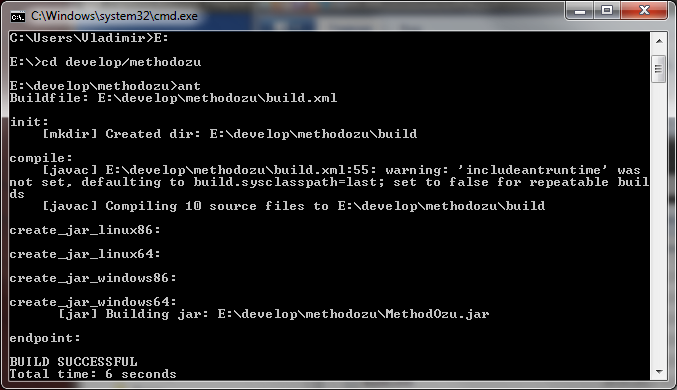
\includegraphics[width=0.8\textwidth]{images/windows-compile.png}
\end{figure}

    После завершения подготовительных операций в Eclipse должна быть доступна вкладка Hadoop Services.
\begin{figure}[h]
    \centering
    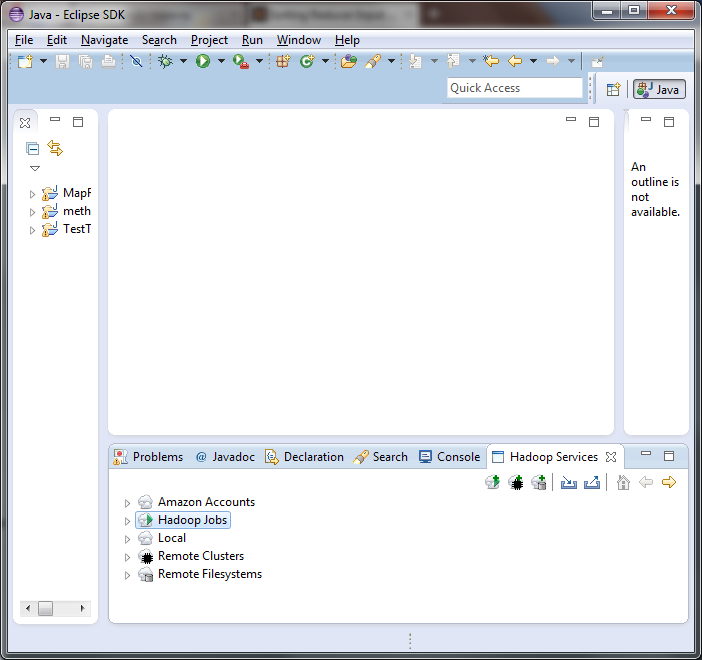
\includegraphics[width=0.65\textwidth]{images/eclipse-hadoop-services.png}
\end{figure}

\clearpage\newpage
    Вызвав окно консоли и перейдя в папку с проектом запускаем компиляцию командой ant. Результатом будет каталог /build и jar файл "MethodOzu.jar".

    Далее работаем с eclipse. В Hadoop Services создаём New Job, выбрав правой клавишей мыши Hadoop Jobs. Следуем инструкциям. 
\begin{figure}[h]
    \centering
    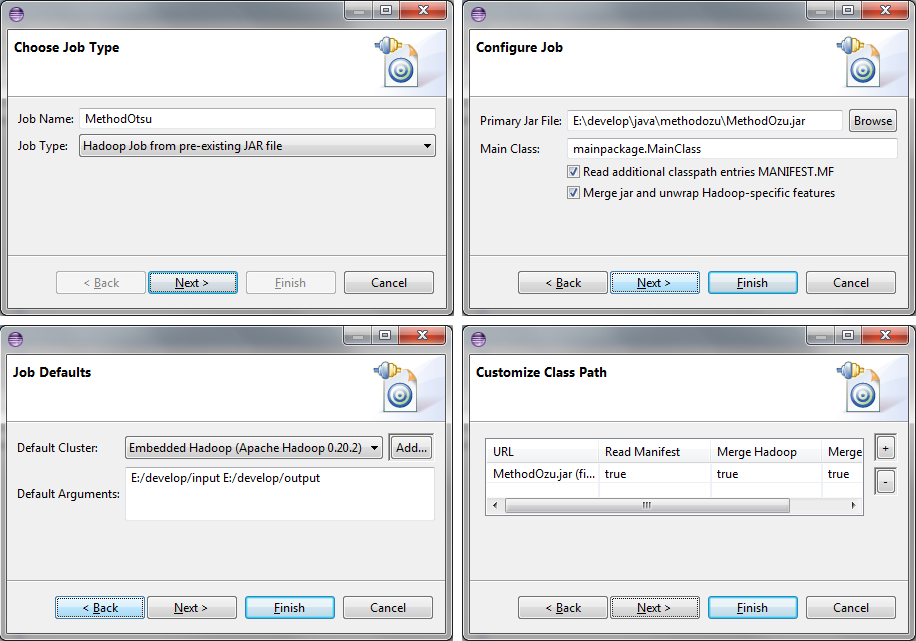
\includegraphics[width=\textwidth]{images/eclipse-create-job.png}
\end{figure}

    Перед запуском необходимо предварительно убедиться, что существует указанный каталог /input и не существует /output и /tmp (может остаться в случае частичного завершения работы программы).

    После запуска обработанные изображения будут сохраняться в указанный /output.
\begin{figure}[h]
    \centering
    
\includegraphics[width=0.6\textwidth]{images/charlie.png}
\end{figure}

\clearpage\newpage
\subsection{Компиляция и запуск под Linux}

    Чтобы скомпилировать и запустить проект необходимо установить Apache ant, настроить Apache Hadoop (см. Настройка оборудования, раздел \ref{sec:TuningCluster}).

    Копируем изображения в папку /input. Убедившись что сервер запущен, а \$HADOOP\_HOME указывает на каталог установленного сервера (echo \$HADOOP\_HOME), запускаем один из скриптов buildrun.sh (компиляция и запуск), либо run.sh (запуск).

    Результат будет находится в hdfs в каталоге /user/hduser/method-otsu-out.

\subsection{Установка ant под Linux}
\begin{lstlisting}
    sudo apt-get update 
    sudo apt-get install ant
\end{lstlisting}

\newpage
\section{Описание среды}

\subsection{Классификация версий Apache Hadoop}
\begin{itemize}
    \item[] 1.0.X ---  текущая стабильная версия, 1.0 release
    \item[] 1.1.X  ---  текущая бета версия, 1.1 release
    \item[] 2.X.X  ---  текущая альфа версия
    \item[] 0.23.X  ---  то же, что и 2.X.X без NN HA.
    \item[] 0.22.X  ---  модули безопасности 
    \item[] 0.20.203.X  ---  старая legacy стабильная версия
    \item[] 0.20.X  ---  старая legacy версия
\end{itemize}


\subsection{Версии использованного программного обеспечения} \label{sec:envsoft}
\begin{itemize}
    \item[] Apache Ant(TM) version 1.9.0 compiled on March 5 2013,
    \item[] Hadoop 1.0.4,
    \item[] Karmasphere Hadoop MapReduce 0.20.203,
    \item[] Ubuntu 11.10, Ubuntu 12.04 i386,
    \item[] Windows 7 x64,
    \item[] Eclipse 4.2.2,
    \item[] javacv-0.4 (javacv-0.4-bin.zip, javacv-0.4-cppjars.zip).
\end{itemize}

\subsection{Известные проблемы}
\begin{enumerate}
    \item Запуск в Karmasphere. Если в пути к /input (и /output) том диска указан заглавной буквой, например E:/develop/input, а не e:/develop/input, то временный каталог /tmp не удалится.
\end{enumerate}


\lstset{basicstyle=\small, backgroundcolor=\color{white}, showstringspaces=false, showspaces=false, numbers=left, numbersep=5pt, commentstyle=\color{mygreen}, breaklines=true, tabsize=2, numberstyle=\color{mygray}}
\newpage\clearpage
\section*{ПРИЛОЖЕНИЕ A\\ Исходный код функций}
\addcontentsline{toc}{section}{Приложение A Исходный код функций}\label{inc:source}
\small
\sloppy
\subsection*{MainClass.java}
\lstinputlisting[language=Java]{../src/mainpackage/MainClass.java}
\subsection*{Histogram.java}
\lstinputlisting[language=Java]{../src/mainpackage/Histogram.java}
\subsection*{ThreshApply.java}
\lstinputlisting[language=Java]{../src/mainpackage/ThreshApply.java}
\subsection*{ImageInputFormat.java}
\lstinputlisting[language=Java]{../src/edu/vt/input/ImageInputFormat.java}
\subsection*{ImageRecordReader.java}
\lstinputlisting[language=Java]{../src/edu/vt/input/ImageRecordReader.java}
\subsection*{LongArrayWritable.java}
\lstinputlisting[language=Java]{../src/edu/vt/io/LongArrayWritable.java}
\subsection*{Image.java}
\lstinputlisting[language=Java]{../src/edu/vt/io/Image.java}
\subsection*{ImageOutputFormat.java}
\lstinputlisting[language=Java]{../src/edu/vt/output/ImageOutputFormat.java}
\subsection*{ImageRecordWriter.java}
\lstinputlisting[language=Java]{../src/edu/vt/output/ImageRecordWriter.java}
\subsection*{WindowInfo.java}
\lstinputlisting[language=Java]{../src/edu/vt/io/WindowInfo.java}
\subsection*{build.xml}
\lstinputlisting[language=XML]{../build.xml}
\subsection*{buildrun.sh}
\lstinputlisting[language=sh]{../buildrun.sh}
\subsection*{run.sh}
\lstinputlisting[language=sh]{../run.sh}
%\subsection*{block.cpp}
%\lstinputlisting[language=C++]{liitings/block.cpp}
%\subsection*{eigen\_m.cpp}
%\lstinputlisting[language=C++]{listings/eigen_m.cpp}
\end{document}
